Total Variation\subsection{Example: Thermal Conductivity on a 1D Heat Rod}\label{ex:heat-set-sample-accuracy}

Consider the one-dimensional heat equation with homogeneous Neumann boundary conditions on the unit interval presented in \ref{ex:heat-set-sample}.


The quantities of interest we study are four point-evaluations of the state variable, at spatial location 0.25, 0.51, 0.67, and 0.98 along the rod.
Choosing any pair of them for the inversion yields six possible quantities of interest maps.
As before, we demonstrate that some choices appear to have advantages over others.

From the prior examples, we would suspect that choosing the QoI map with lower skewness results in lower Total Variations.
However in the earlier experiments we utilized maps that inverted into sets of identical size, which is not the case in this nonlinear example; each QoI map scales sets differently depending on the location in the parameter space.
To isolate this scaling effect, we attempt to compare QoIs that invert into sets of similar size \emph{on average} but have differing average skewness.

This is what motivated our specific choice of spatial locations at which to measure the state variable $T$.
Our first QoI $\qoiA$ uses measurements at 0.25 and 0.51, and has average skewness of 1.08, and our second $\qoiB$ uses measurements at 0.67 and 0.98, with average skewness 1.56.
While we would have liked to use a map with average skewness of 2 for a more similar comparison to the prior examples, this was the best range we could find where the maps inverted into sets of comparable size on average\footnote{average local scaling is $1.99$ for $\qoiA$ and $2.19$ for $\qoiB$.}.

Owing to the nonlinearity of the problem, the Total Variations between reference and estimated probability measures now have an inherent dependence on the location of the point $\param$ in the parameter space.
We ran the simulations for a regular $3\times3$ grid exploring the interior of the parameter space and present two of the nine reference points that illustrate the differences in the nonlinear case from the linear examples.
Most notably, the location of truth will impact our ability to approximate the solution to the SIP. 

In the two-dimensional data spaces $\dspaceA$ and $\dspaceB$, our uncertainty is a uniform box centered at $\qoiA(\paramref)$ with side-lengths of 0.1.
When $\paramref$ is the bottom-left corner of our $3\times3$ grid, the two maps produce very different results, with $\qoiA$ outperforming $\qoiB$ in a similar manner as we saw in the linear examples (see Fig.~\ref{fig:NLbotleft}).
When $\param_{\text{ref}}$ is in the upper-center of the grid, the inverse images are similar, as shown in Fig.~\ref{fig:NLtopmid}, and so which map to use forinversion into this part of the parameter spaces is not a clear choice. We might even be tempted to use the more-skewed (on average) map since it inverts into a set with smaller support.


\begin{figure}[h]
  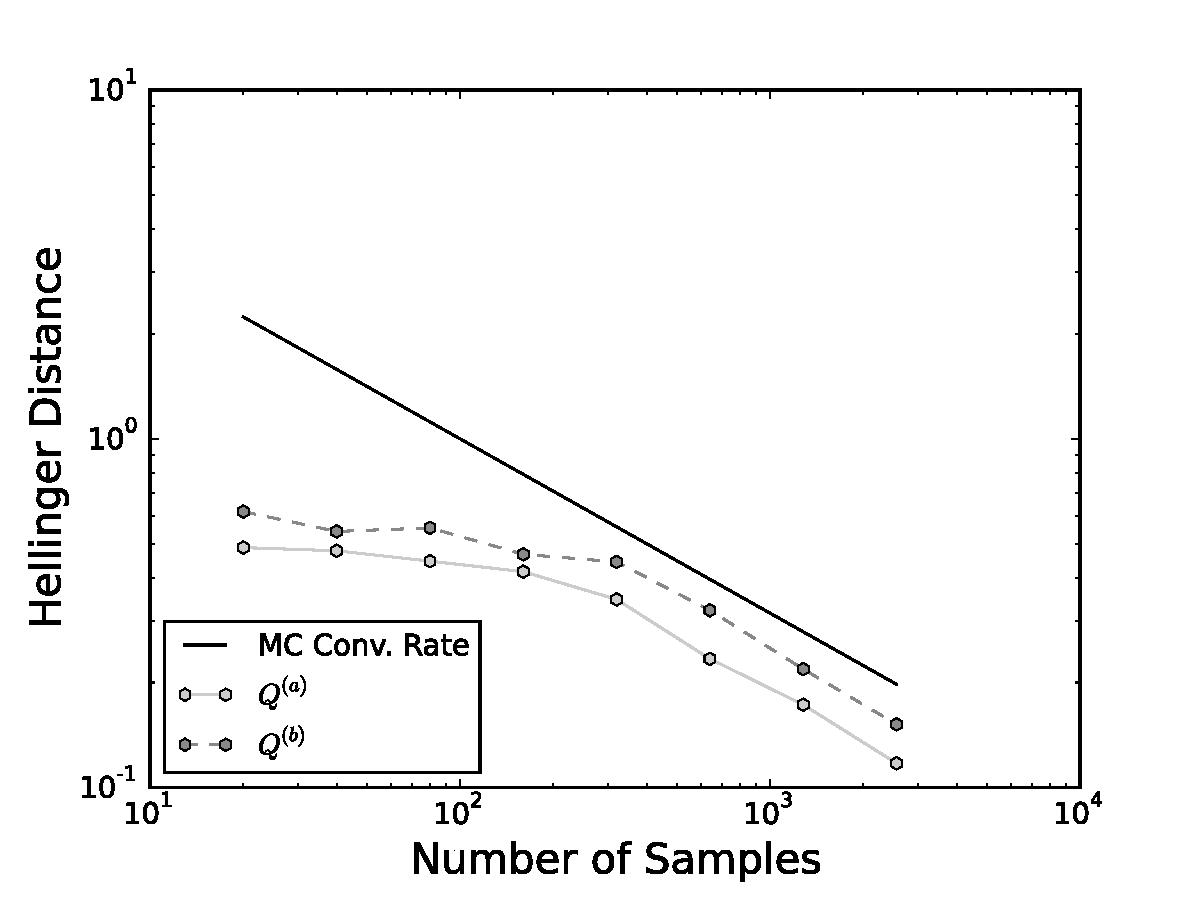
\includegraphics[width=\linewidth]{./images/pt0Plot-reg_BigN_40000_reg_M_1_rand_I_100000}
  \caption{Convergence in TV metric for the bottom left reference value in a 3x3 grid in $\pspace$. There is a notable difference in the accuracy of the measure recovered depending on which QoI map is used.}
  \label{fig:NLbotleft}
\end{figure}

\begin{figure}[h]
  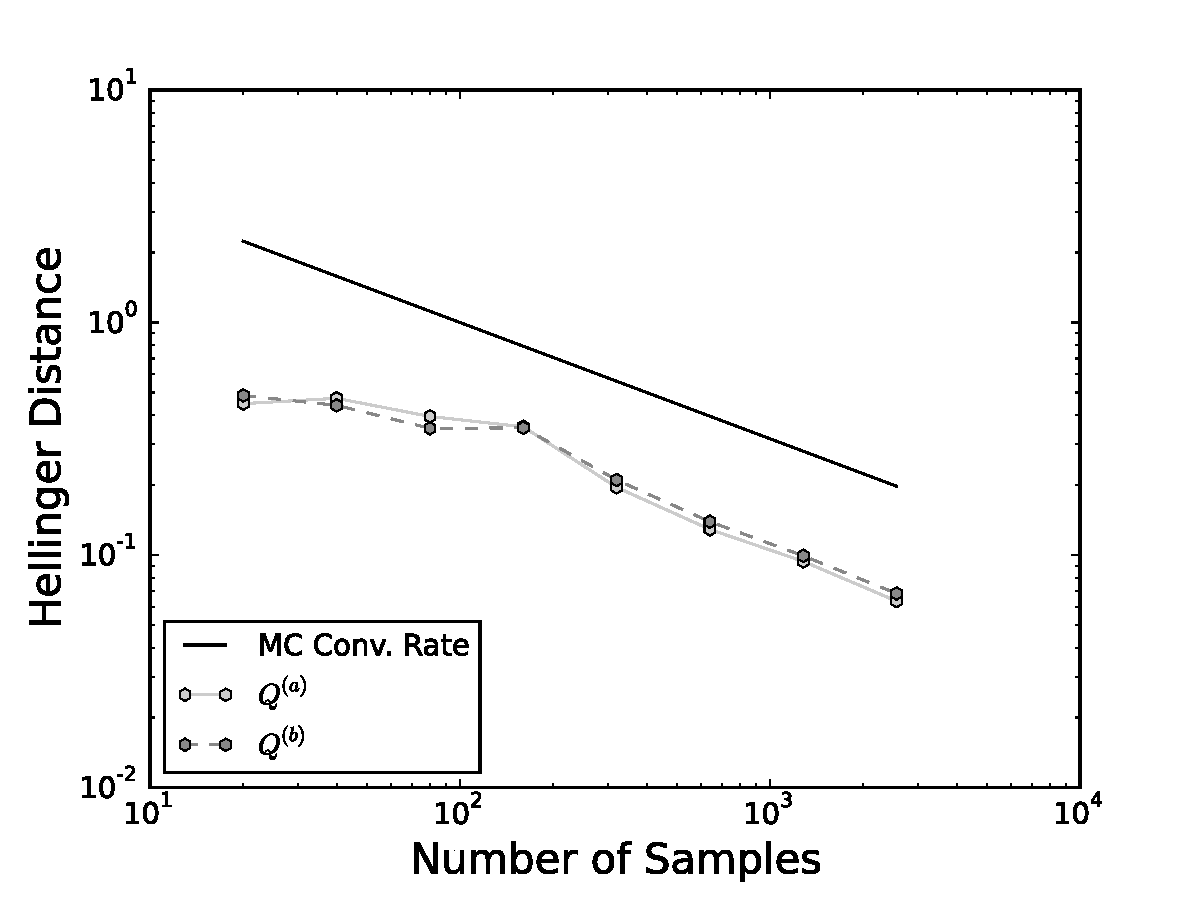
\includegraphics[width=\linewidth]{./images/pt5Plot-reg_BigN_40000_reg_M_1_rand_I_100000}
  \caption{Convergence in TV metric for the top-middle reference value in a 3x3 grid in $\pspace$. For this value of truth, there is no distinguishable difference between the solutions that come from using either QoI map. The location in parameter space of truth will impact how sensitive experimental designs are to approximation errors in limited exploration of $\pspace$.}
  \label{fig:NLtopmid}
\end{figure}


Of the nine reference $\param$'s we studied, $\qoiA$ yielded no considerable advantage in terms of the number of samples required to approximate the inverse images in three cases (the plots were similar to that in the right of Fig.~\ref{fig:NLHD}).
In three cases, $\qoiA$ performed better than $\qoiB$, (somewhere between the two figures in Fig.~\ref{fig:NLHD}).
In two cases, $\qoiA$ performed better than  $\qoiB$, as in the left of Fig.~\ref{fig:NLHD}.
In one case (with $\param$ in the bottom right corner), the difference was even more dramatic ($\qoiA$ yielded similar Total Variations with less than a fourth the samples).

\begin{figure}
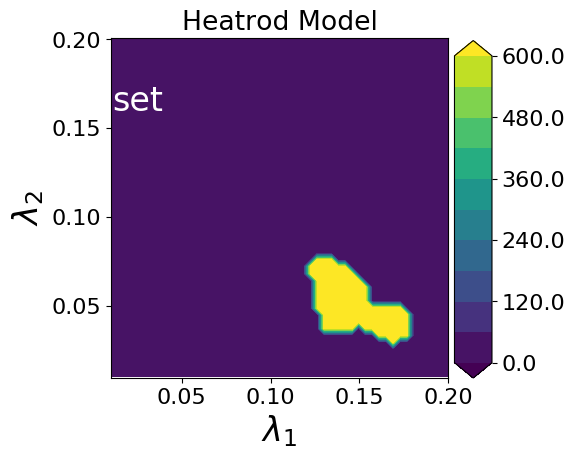
\includegraphics[width=.45\linewidth]{examples/fig_heatrod_q1/HeatrodModel--set_N50_em.png}
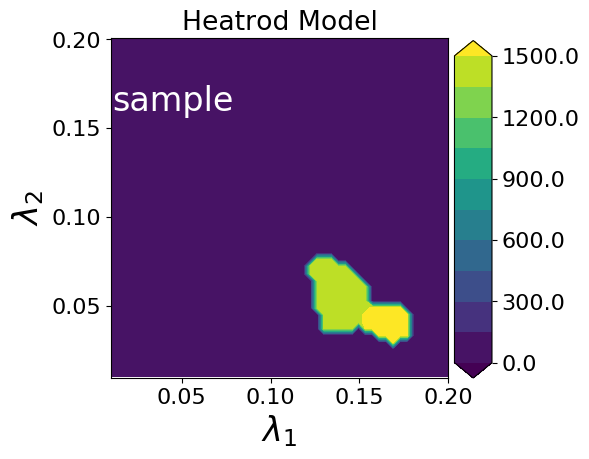
\includegraphics[width=.45\linewidth]{examples/fig_heatrod_q1/HeatrodModel--sample_N50_mc.png}

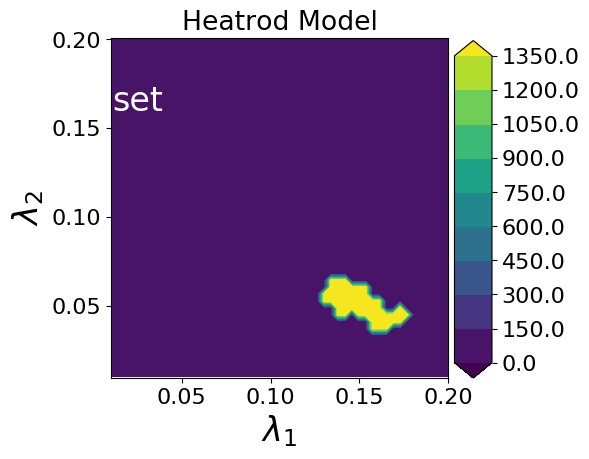
\includegraphics[width=.45\linewidth]{examples/fig_heatrod_q1/HeatrodModel--set_N500_em.png}
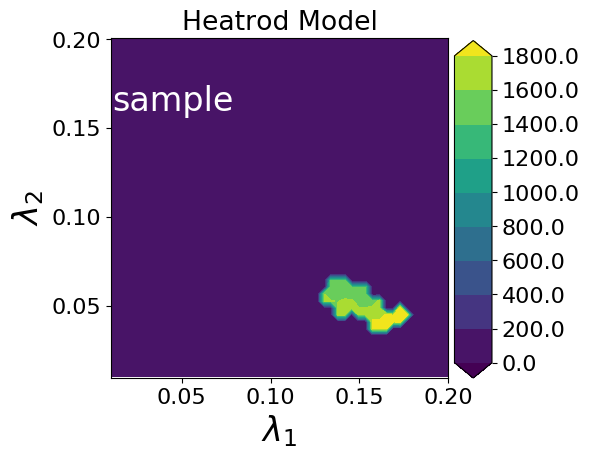
\includegraphics[width=.45\linewidth]{examples/fig_heatrod_q1/HeatrodModel--sample_N500_mc.png}

\caption{The inverse image of the reference measure for $\qoiA$ for $\nsamps = 50$ (top) and $\nsamps = 500$ (bottom). }
\label{fig:heatrod-convergence-a}
\end{figure}

\begin{figure}
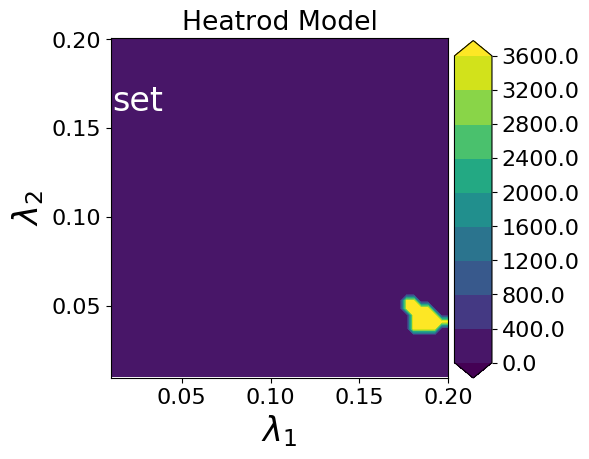
\includegraphics[width=.45\linewidth]{examples/fig_heatrod_q2/HeatrodModel--set_N50_em.png}
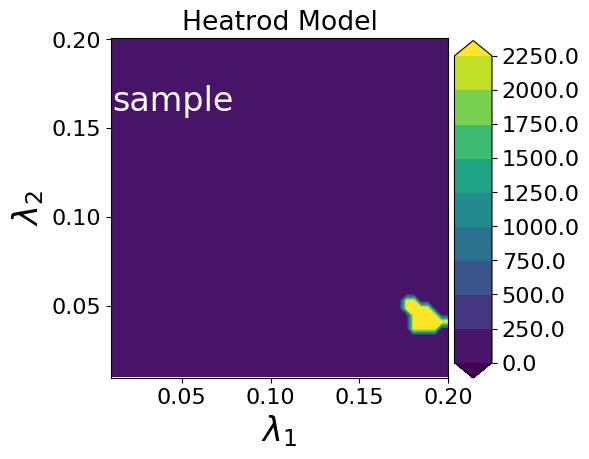
\includegraphics[width=.45\linewidth]{examples/fig_heatrod_q2/HeatrodModel--sample_N50_mc.png}

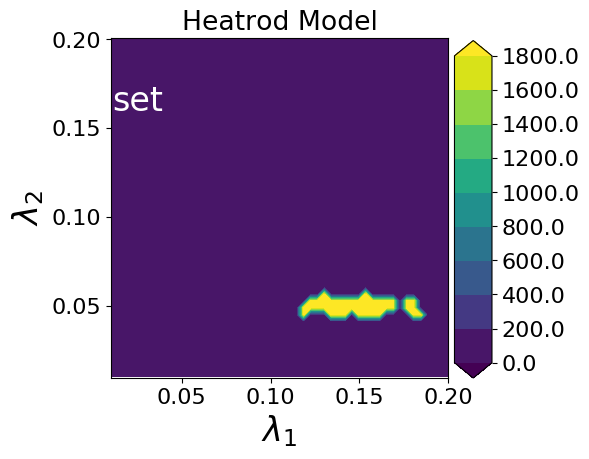
\includegraphics[width=.45\linewidth]{examples/fig_heatrod_q2/HeatrodModel--set_N500_em.png}
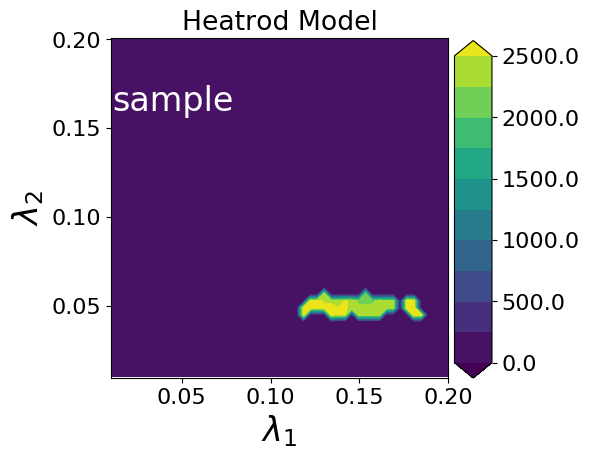
\includegraphics[width=.45\linewidth]{examples/fig_heatrod_q2/HeatrodModel--sample_N500_mc.png}

\caption{The inverse image of the reference measure for $\qoiB$ for $\nsamps = 50$ (top) and $\nsamps = 500$ (bottom). TK - need to remark about how this map may be more precise but it makes it harder to identify the set that contains truth when few model evaluations are available to us (low $\nsamps$). }
\label{fig:heatrod-convergence-b}
\end{figure}


These results motivate further study into utilizing different QoI maps (perhaps some of those other four combinations available to us in this example) depending on where the samples came from in the parameter space.
In general, we saw in this example that given that two maps invert into sets of similar size on average, using the one with lower skewness results in less samples required to accurately approximate the inverse image.
The maps we used had average skewnesses that differed by 0.5 (instead of by 1), and the trend from the linear examples still held in significant portions of the parameter space.
